
\section{Tools Used}

\subsection{Modeling \& Simulation}\label{intro:sim}

Supply and demand in nuclear fuel cycle simulation drives the flow of resources
between entities and is the primary entity interaction mechanism. The supply and
demand of a given fuel cycle becomes highly complex when including the recycling
of material. Even with such a complication, the notion of a generic fuel cycle,
i.e., from the perspective of facilities that supply and demand material,
quickly begins to look like a supply chain model. There is a growing literature
of agent-based supply chain modeling
\cite{swaminathan_modeling_1998,julka_agent-based_2002,van_der_zee_modeling_2005,chatfield_multi-formalism_2007,holmgren_agent_2007}.
The general premise of these types of models is that individual facilities have
a notion of their needs (i.e., their demands) and can express to the system
these needs at the required time. There is heavy use of inventory policy to
determine the correct amount of material inventory that is needed and the
correct time to request a resupply. Such an approach has not heretofore been
attempted for the nuclear fuel cycle and would support a variety of use
cases. For example, reactor facilities could be allowed to be fueled by multiple
fuel types (e.g., UOX or MOX), and decide which type to choose based on the
simulation environment.

The notion of social modeling in fuel cycle simulation, e.g., employing regional
bias, has to date been a secondary concern. Some semblance of this capability is
needed if one is to incorporate outside effects on a domestic fuel cycle
model. Furthermore, a robust capability is required if one wishes to actually
investigate dynamic interactions between regional entities. Again, a full
treatment of this sort of regional interaction would require international
relations models, most of which can be found in the cross-cutting disciplines of
economics, political science, and game theory. The primary solution technique in
game theory is Nash Equilibrium. It describes an optimal solution as follows:
given a set of players, states, preferences, and actions, all players choose an
action such that any single player's deviation from that actions results in a
state of lower preference for that player (thus no player has an incentive to
deviate) \cite{mccarty_political_2007}. There also exists a body of literature
that examine Nash Equilibria in the context of optimal flow models
\cite{mazumdar_fairness_1991,nagurney_supply_2002,song_nash_2002}. However, the
complexity of such models quickly brings them out of the scope of our needs,
i.e., dynamic modeling of multi-lateral scenarios ranging 100+ years in a
``reasonable'' amount of computation time. Accordingly, a market resolution
mechanism is proposed that allows for interaction amongst the various facilities
and managing entities (e.g., their regions). In order to inform a cardinal
preference \cite{strotz_cardinal_1953} relation for a facility over its possible
supply materials.

\subsection{Transportation Problems \& Mathematical Programming}\label{intro:prog}

The previous sections have outlined a specific need for nuclear fuel cycle
simulation: determining the flow of resources in a system of supply and demand,
given a variety of possible capacities and informed by economic and social
models. Constrained network flow determination is a canonical problem in
computer science and operations research. Further, there is a rich history and
capability of modeling such problems using mathematical programming.

A network flow model is represented by a graph, $G(N, A)$, comprised of nodes
$N$ and arcs $A$. If flow can occur between some node $i$ and some other node
$j$, then it flows along arc $(i, j)$. An example of a network-flow graph is
shown in Figure \ref{fig:node-arcs}.

\begin{figure}[H]
  \begin{center}
    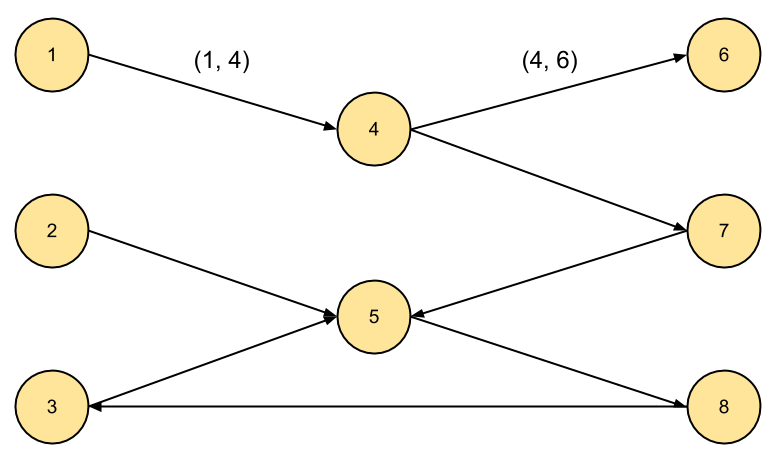
\includegraphics[height=7.5cm]{./chapters/1-intro/figs/node-arcs.png}
  \caption{An example node-arc network configuration. Arrows denote possible
    flow directions. Arc notation examples are provided for arcs (1,4) and
    (4,6).}
  \label{fig:node-arcs}
  \end{center}
\end{figure}

Given a graph instance, an optimal flow between nodes can be found provided
\textit{objective coefficients} and \textit{constraints}. \textit{Decision
  variables} for this optimization problem comprise the optimal \textit{flow
  assignment}. If all decision variables are linear, then the resulting
formulation is termed a Linear Program (LP), and can be solved using related
techniques. A full discussion of LPs and their solution techniques is provided
in Appendix \ref{app:lp}. If any decision variables are integer, then the
resulting formulation is termed a Mixed-Integer Linear Program (MILP). For
instance, binary variables can be used in network-flow problems to denote
whether an arc has flow or not. A full discussion of MILPs and their solution
techniques is provided in Appendix \ref{app:ip}. Many different types of
problems can be solved using this structure. For the purposes of this work
\textit{transportation} problems, a specialization of the network-flow problems,
are utilized.

Transportation problems model the flow of a commodity between source nodes and
sink nodes. Critically, this simplification allows for the nodes in the
transportation problem to be categorized into two explicit groups, sources and
sinks. In other words, source nodes and sink nodes comprise two distinct
subsets, $N_1, N_2$, the union of which comprises all nodes in the
transportation graph, $N$. These properties can be described in set notation.

\begin{equation}
  N_1 \subset N
\end{equation}

\begin{equation}
 N_2 \subset N
\end{equation}

\begin{equation}
  N_1 \cup N_2 = N
\end{equation}

From the node-arc graph point of view, this strict subset division allows for
the transportation problem to be modeled as a \textit{bipartite} graph.

\begin{figure}[H]
  \begin{center}
    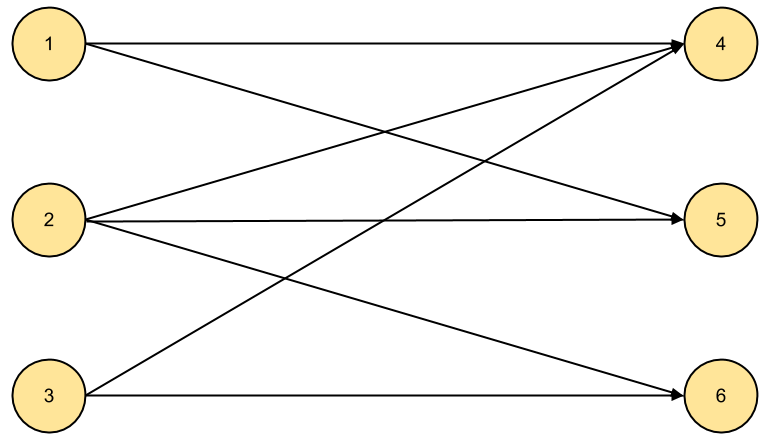
\includegraphics[height=7.5cm]{./chapters/1-intro/figs/node-arcs-bipartite.png}
  \caption{An example node-arc transportation network configuration. Arrows
    denote possible flow directions. Note that all nodes either belong to the 
    set of sources (left) or set of sinks (right).}
  \label{fig:node-arcs-bipartite}
  \end{center}
\end{figure}

The transportation problem is a platform on which one can model more general
problems. The minimum-cost transportation problem is a useful example. In such a
formulation, each arc has an associated \textit{unit cost} associated with the
cost of transporting a unit of a commodity along it, $c_{i,j}$. Additionally,
supplier and consumer nodes have an associated supply, $s_i$, or demand, $d_i$,
which provide a notion of \textit{node capacity}. The minimum-cost
transportation problem can be formulated as a linear program as shown in
Equation \ref{eqs:xport}.

%%% 
\begin{subequations}\label{eqs:xport}
  \begin{align}
    %%
    \min_{x} \:\: & 
    \sum_{(i, j) \in A} c_{i,j} x_{i,j}
    & \label{eqs:xport_obj} \\
    %%
    \text{s.t.} \:\: &
    \sum_{j \in N_2} x_{i,j} \leq s_i
    & \forall i \in N_1  \\
    %%
    &
    \sum_{i \in N_1} x_{i,j} \geq d_i
    & \forall j \in N_2  \\
    %%
    &
    x_{i,j} \geq 0
    & \forall (i, j) \in A \label{eqs:xport_x}
    %%
  \end{align}
\end{subequations}
%%% 

As is noted in many texts, an intuitive constraint on the problem to guarantee a
feasible solution is that the total demand in the system must be no greater than
the total supply in the system, shown in Equation \ref{eqs:xp_constr}.

\begin{equation}\label{eqs:xp_constr}
  \sum_{j \in N_2} d_j \leq \sum_{i \in N_1} s_i
\end{equation}

\noindent
Feasibility in this sense can be guaranteed by adding an artificial supply
node. Such a node can have infinite supply capacity but at (effectively)
infinite cost. The problem can then be solved, and any flow leaving the
artificial node in the optimal solution can be dealt with accordingly, e.g., it
can be ignored.

A more complex transportation-problem formulation can support systems in which
supply or demand can be met by multiple commodities.  Variables and constants in
the multi-commodity formulation are generally analogs of their counterparts in
the single-commodity problem. There is a unit cost $c_{i,j}^{h}$ for commodity
$h$ to traverse arc $(i,j)$. A supplier of commodity $h$ has a certain supply
capacity $s_i^h$ which cannot be surpassed and demanders of commodity $h$ have a
certain demand level which must be met, $d_i^h$.

In the simplest extension from the single-commodity to multi-commodity
transportation problem, arc constraints for all commodities are combined, i.e.,
for a given arc $(i, j)$, there is a single capacity $u_{i,j}$. A classic
interpretation of this enhanced complexity deals with data networks. Multiple
classifications of data exist, but they all must traverse the same network
infrastructure. Accordingly, the infrastructure can only accommodate a certain
level of total flow among all communication types. The formulation of the
multi-commodity flow problem is shown in Equation \ref{eqs:MCTP}. Note the
commodity coupling in Equation \ref{eqs:MCTP_cap}.

%%% 
\begin{subequations}\label{eqs:MCTP}
  \begin{align}
    %%
    \min_{x} \:\: & 
    \sum_{i \in I}\sum_{j \in J}\sum_{h \in H} c_{i,j}^{h} x_{i,j}^{h}
    & \label{eqs:MCTP_obj} \\
    %%
    \text{s.t.} \:\: &
    \sum_{j \in J} x_{i,j}^{h} \leq s_{i}^{h}
    &
    \forall \: i \in I, \forall \: h \in H \label{eqs:MCTP_sup} \\
    %%
    &
    \sum_{i \in I} x_{i,j}^{h} \geq d_{j}^{h}
    & 
    \forall \: j \in J, \forall \: h \in H \label{eqs:MCTP_dem} \\
    %%
    &
    \sum_{h \in H} x_{i,j}^{h} \leq u_{i,j}
    & 
    \forall \: j \in J \label{eqs:MCTP_cap} \\
    %%
    &
    x_{i,j}^{k} \geq 0
    &
    \forall \: i \in I, \forall \: j \in J, \forall \: h \in H \label{eqs:MCTP_x}
    %%
  \end{align}
\end{subequations}
%%% 

It is possible to reduce instances of the multi-commodity transportation
problem. In the case in which is no arc that shares multiple commodities, the
multicommodity connection constraints disappear, and the single multi-commodity
problem can be broken into $m$ different single-commodity transportation
problems, where $m$ is the cardinality of the set of commodities, $H$. Such
reductions are important because optimization problems will generally scale
poorly with problem size.

Optimization problems are solved by solving a number of decision
problems. Decision problems are generally computationally
\textit{hard}. Decision problems ask yes or no questions, e.g., ``is there a
flow path that with a flow larger than $x$?''. An optimization problem asks
instead ``what is the flow path with the largest flow?''. Any problem can be
associated with one of four categories of computational complexity:
Polynomial-time ($\mathcal{P}$), Nondeterministic Polynomial-time
($\mathcal{NP}$), Nondeterministic Polynomial-time Complete ($\mathcal{NP}$-C),
and Nondeterministic Polynomial-time Hard ($\mathcal{NP}$-hard). A classic
example of a polynomial-time algorithm is naive matrix inversion, known to be of
order $n^3$ (i.e., $\mathcal{O}(n^3)$) for a given $n \times n$ matrix.

A decision problem, on the other hand, is considered to be in ($\mathcal{NP}$)
if for any proposed solution, there is a \textit{short certificate}.

\begin{define}
A \textbf{certificate} is a method to verify that a solutions provides a
positive or negative response to the question at hand. A certificate is
considered \textbf{short} if it is polynomial in size and can be verified in
polynomial time.
\end{define}

\noindent
A decision problem, $Q$, is considered to be in $\mathcal{NP}$-C, if $Q \in
\mathcal{NP}$ and \textit{any} problem, $P \in \mathcal{NP}$ is polynomial-time
reducible to $Q$. That is, instances of $P$ can be reformulated as instances of
$Q$ in polynomial time. The most popular candidate of this polynomial reduction
is the Satisfiability Problem, known to be in $\mathcal{NP}$-C
\cite{Cook:1971:CTP,levin1973universal}. Finally, a problem $Q$, is in
$\mathcal{NP}$-hard, if any problem $P \in \mathcal{NP}$ is polynomial-time
reducible to $Q$, but $Q \not\in \mathcal{NP}$. If a decision problem is in
$\mathcal{NP}$-C, then the corresponding optimization problem is
$\mathcal{NP}$-hard. The various levels of complexity are related. The
relationship between these set of problem complexities, reflecting current
understanding, is shown graphically in Figure \ref{fig:complexity}.

\begin{figure}[H]
  \begin{center}
    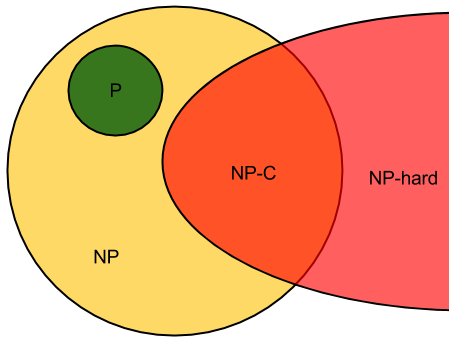
\includegraphics[height=7.5cm]{./chapters/1-intro/figs/complexity.png}
  \caption{The relationship between the various types of problem complexities.}
  \label{fig:complexity}
  \end{center}
\end{figure}

Certain optimization problems can be solved with specialty algorithms that
greatly decrease solution times. However, because optimization problems are
$\mathcal{NP}\text{-hard}$, no guarantee can be made \textit{in general}
regarding their scalability. Worst case scenarios result in exponential scaling
with problem size. Further, in practice, MILPs experience much worse solution
time behavior than do LPs. In short, reducing problem size is an important
strategy for solving optimization problems more quickly.
